\documentclass{article}
\usepackage[UTF8]{ctex}
\usepackage{geometry}
\usepackage{makecell}
\usepackage{amsmath}
\usepackage{graphicx}
\usepackage{subcaption}

\geometry{a4paper,scale=0.75}

\title{\heiti 实验十\ 气垫上弹簧振子的简谐振动}
\author{\kaishu 田睿轩\ 物理学院\ 1900011602}
\date{2020年11月14日}
\newcommand{\degree}{^\circ}

\begin{document}
    \maketitle

    \section{实验内容、数据处理与结论}

    \subsection{弹簧振子振动周期与振幅的关系}
    
    将弹簧振子设置成不同振幅,即将弹簧振子从到平衡位置不同距离处释放,在其第一次回到平衡位置时开始计时,
    第三次回到平衡位置时结束计时,之间的时间差作为弹簧振子的周期。实验中,振幅分别设置为$10cm$,$20cm$,
    $30cm$,$40cm$,分别测量从左侧释放和从右侧释放的周期,对于同一个振幅,左右各测三组周期,然后取平均值作为该振幅下的周期。

    测量周期使用光电门传感器,实验中将光电门传感器置于振子的平衡位置。若测从左侧释放的振动周期,则
    在调整光电门位置的时候应从右侧移动光电门靠近处于平衡位置的振子上的挡光片,当仪器检测到光被挡住时即
    停止移动,将光电门固定。

    实验中测得的数据如下表所示:

    \begin{center}
        \begin{tabular}{|c|c|c|c|c|c|c|c|}
            \hline
            $A(cm)$ & \multicolumn{3}{|c|}{$T_{\text{左}}(s)$} & \multicolumn{3}{|c|}{$T_{\text{右}}(s)$} & $T(s)$ \\
            \hline
            10.00 & 1.91532 & 1.91520 & 1.91550 & 1.91548 & 1.91565 & 1.91540 & 1.91543\\
            \hline
            20.00 & 1.91896 & 1.91890 & 1.91924 & 1.91921 & 1.91919 & 1.91939 & 1.91915\\
            \hline
            30.00 & 1.92134 & 1.92161 & 1.92150 & 1.92176 & 1.92188 & 1.92191 & 1.92167\\
            \hline
            40.00 & 1.92292 & 1.92302 & 1.92335 & 1.92329 & 1.92340 & 1.92341 & 1.92323\\
            \hline
        \end{tabular}
    \end{center}

    对于理想的弹簧振子,振动周期应与振幅无关,但从实验数据中不难得出结论:气垫导轨上的
    弹簧振子,周期随着振幅的增加而增加。这是因为虽然气垫导轨已经相当大程度上的减小了
    摩擦力,但整个振动系统仍不可避免地存在阻尼,这种阻尼降低了振子的运动速度,并且
    振幅越大,阻尼做功越多,于是周期便随着振幅的增加而增加。

    \subsection{弹簧振子振动周期与振子质量的关系}

    固定弹簧振子的振幅为$40cm$,通过在振子上安装骑码来改变振子的质量(骑码的质量通过天平测得),
    测量不同质量的弹簧振子的振动周期,进而研究周期与质量的关系。

    实验中对于同一质量的弹簧振子,分别从左侧和右侧释放,每一侧测量三次周期,取平均作为
    该振子质量下的振动周期。

    实验数据如下表所示:

    \begin{center}
        \begin{tabular}{|c|c|c|c|c|c|c|c|c|}
            \hline
            $m_1(g)$ & \multicolumn{3}{|c|}{$T_{\text{左}}(s)$} & \multicolumn{3}{|c|}{$T_{\text{右}}(s)$} & $T(s)$ & $T^2(s^2)$\\
            \hline
            460.53 & 1.92294 & 1.92318 & 1.92331 & 1.92331 & 1.92348 & 1.92336 & 1.92326 & 3.69893\\
            \hline
            514.09 & 2.03042 & 2.03043 & 2.03049 & 2.03059 & 2.03060 & 2.03047 & 2.03050 & 4.12293\\
            \hline
            565.18 & 2.12767 & 2.12768 & 2.12772 & 2.12797 & 2.12796 & 2.12788 & 2.12781 & 4.52758\\
            \hline
            617.13 & 2.22215 & 2.22208 & 2.22223 & 2.22249 & 2.22266 & 2.22253 & 2.22236 & 4.93884\\
            \hline
            665.50 & 2.30692 & 2.30679 & 2.30650 & 2.30711 & 2.30715 & 2.30749 & 2.30699 & 5.32220\\
            \hline
        \end{tabular}
    \end{center}

    绘制$T^2-m_1$关系曲线,如下图所示:
    
    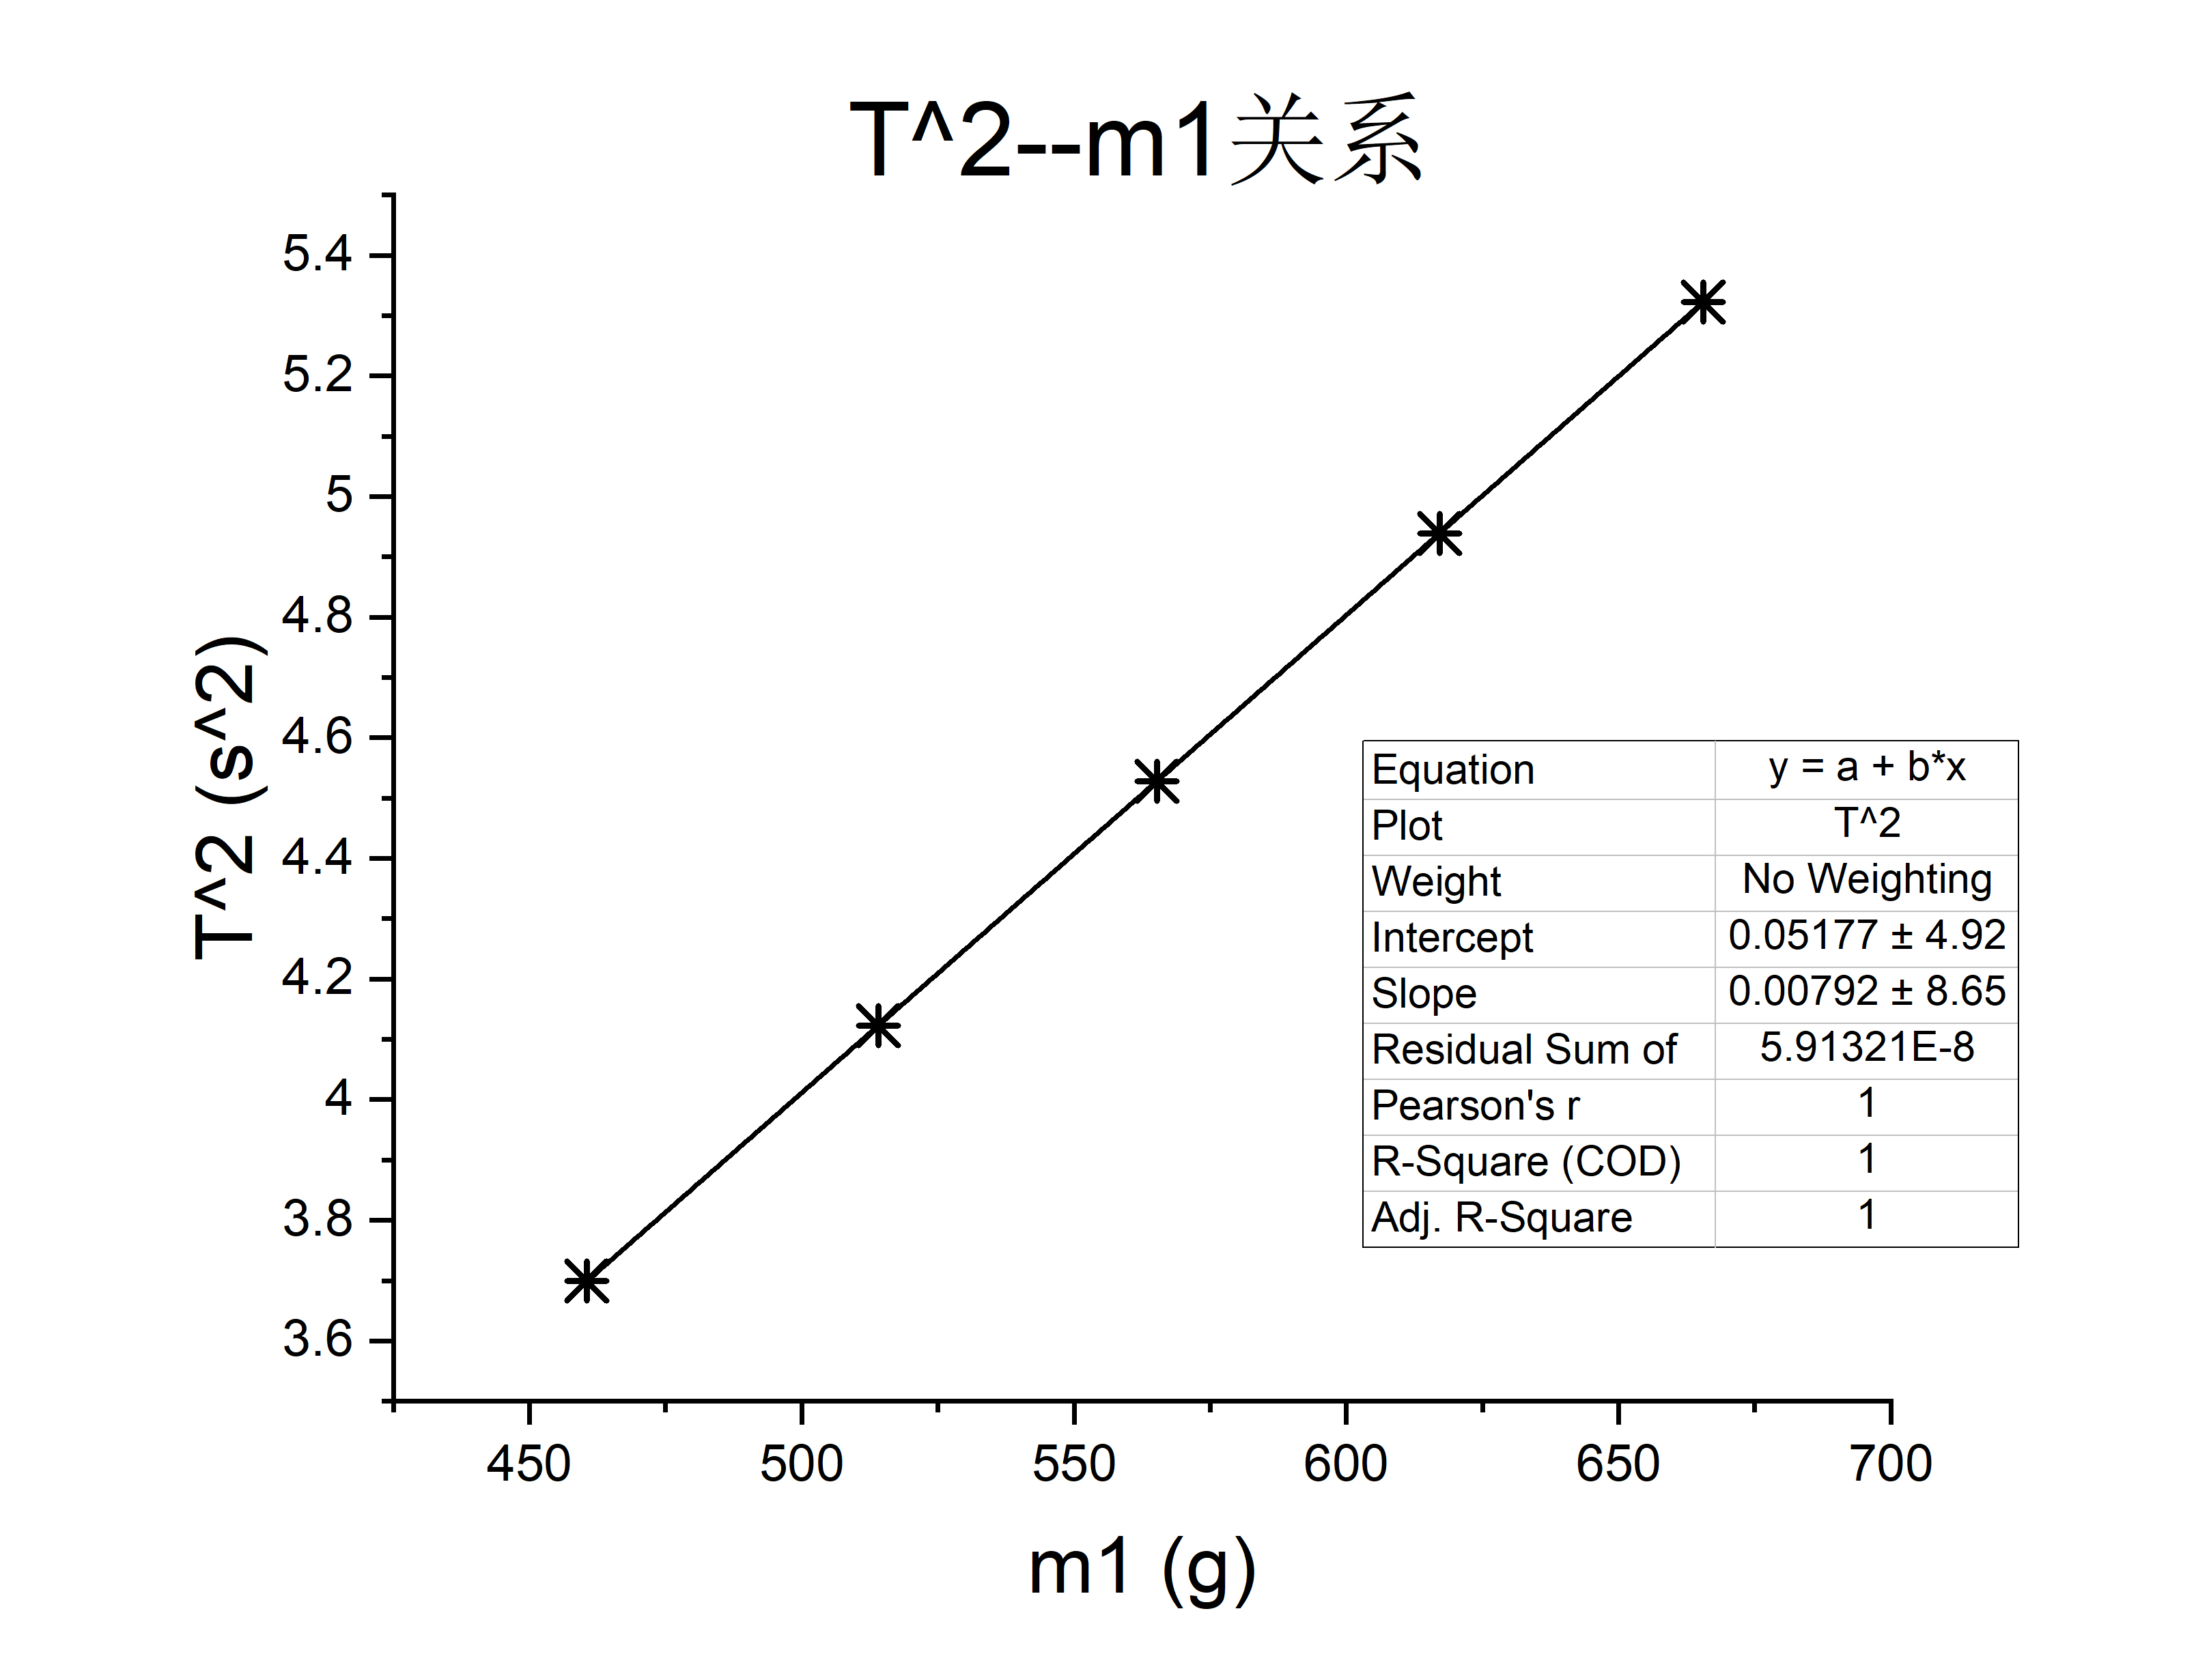
\includegraphics[width=0.85\textwidth]{T^2--m1.jpg}

    可以看出,弹簧振子的振动周期的平方,与振子的质量成正比。根据拟合出的数据直线的斜率$a=0.00791939\ s^2\cdot g^{-1}$,截距$b=0.0517180\ s^2$,相关系数$r=0.99999999857$

    而根据简谐振动的公式,假设系统不存在阻尼,则振动周期满足:
    $$T=2\pi \sqrt{\frac{m_1+m_0}{k}},\ \text{即}T^2=\frac{4\pi^2}{k}m_1+\frac{4\pi^2}{k}m_0$$
    其中$m_1$为振子的质量,$m_0$为弹簧的有效质量,$k$为弹簧的劲度系数。

    因此,$T^2-m_1$关系曲线的斜率$a=\frac{4\pi^2}{k}$,\text{截距}$b=\frac{4\pi^2}{k}m_0$,由此求出:
    $$k=\frac{4\pi^2}{a}=4.98593N/m$$
    $$m_0=\frac{b}{a}=6.530g$$

    下面计算结果的不确定度:

    首先计算斜率和截距的不确定度,然后利用不确定度的传递公式得到$k$和$m_0$的不确定度。其中,斜率的不确定度
    由A类不确定度(直线拟合产生的不确定度)与B类不确定度(变量允差产生的不确定度)方和根构成。
    $$\sigma_{a,A}=a\sqrt{\frac{1/r^2-1}{n-2}}=0.00791939\sqrt{\frac{1/0.99999999^2-1}{3}}=2.0447\times 10^{-7}s^2\cdot g^{-1}$$
    $$\sigma_{a,B}=\frac{e_{T^2} \sqrt{3}}{\sqrt{\sum_{i=1}^5 (x_i-\bar{x})^2}}=\frac{2T\cdot e_T/ \sqrt{3}}{\sqrt{\sum_{i=1}^5 (x_i-\bar{x})^2}}=\frac{2\times 2.30699\times 1\times 10^{-5}/\sqrt{3}}{\sqrt{26322.3}}=1.6419\times 10^{-7}s^2\cdot g^{-1}$$
    $$\sigma_a=\sqrt{\sigma_{a,A}^2+\sigma_{a,B}^2}=2.9453\times 10^{-7}s^2\cdot g^{-1}$$
    $$\sigma_b=\sigma_{T^2}\sqrt{\frac{\bar{x^2}}{\sum_{i=1}^5 (x_i-\bar{x})^2}}=9.3440\times 10^{-5}s^2$$
    $$\sigma_k=k\cdot \frac{\sigma_a}{a}=0.00013N/m$$
    $$\sigma_{m_0}=m_0\sqrt{(\frac{\sigma_a}{a})^2+(\frac{\sigma_b}{b})^2}=0.012g$$

    综上,可得振动系统弹簧的劲度系数和弹簧的等效质量:
    $$k=(4.98503\pm 0.00013)N/m$$
    $$m_0=(6.530\pm 0.012)g$$
    
    \subsection{振动系统机械能与位移的关系}
    测量弹簧振子在第一个四分之一周期内经过不同位移处的速度,进而算出其动能,再根据之前测得的弹簧的劲度系数,
    计算在这些位移处的弹性势能,从而得到不同位移处弹簧振子的机械能。

    实验中使用光电门传感器和U型挡光片测量振子的速度,光电门传感器可以测得U型挡光片两次挡光的时间差,
    用游标卡尺量出挡光片两片挡光板之间的距离,即可算出弹簧振子的速度。

    实验中振幅取$40cm$,振动系统的质量用振子质量和弹簧有效质量的和,即$m=m_1+m_0=467.06g$

    实验中测得的数据如下表所示:

    \begin{center}
        \begin{tabular}{|c|c|c|c|c|c|c|c|c|c|c|}
            \hline
            $x(cm)$ & \multicolumn{2}{|c|}{0.00} & \multicolumn{2}{|c|}{19.50} & \multicolumn{2}{|c|}{28.40} & \multicolumn{2}{|c|}{34.60} & \multicolumn{2}{|c|}{40.00}\\
            \hline
            $\delta t_i(ms)$ & 左 & 右 & 左 & 右 & 左 & 右 & 左 & 右 & 左 & 右\\
            \hline
            $i=1$ & 7.69 & 7.73 & 8.72 & 8.73 & 10.79 & 10.72 & 14.92 & 14.83 & -- & --\\
            \hline
            $i=2$ & 7.70 & 7.74 & 8.73 & 8.74 & 10.79 & 10.73 & 14.93 & 14.88 & -- & --\\
            \hline
            $i=3$ & 7.71 & 7.73 & 8.73 & 8.74 & 10.76 & 10.72 & 14.83 & 14.82 & -- & --\\
            \hline
            平均 & 7.70 & 7.73 & 8.73 & 8.74 & 10.78 & 10.72 & 14.89 & 14.84 & -- & --\\
            \hline
            $\delta S(cm)$ & 0.998 & 1.000 & 0.998 & 1.000 & 0.998 & 1.000 & 0.998 & 1.000 & -- & --\\
            \hline
            $v(m/s)$ & \multicolumn{2}{|c|}{1.295} & \multicolumn{2}{|c|}{1.144} & \multicolumn{2}{|c|}{0.9293} & \multicolumn{2}{|c|}{0.6721} &  \multicolumn{2}{|c|}{0}\\
            \hline
            $E_k(J)$ & \multicolumn{2}{|c|}{0.3916} & \multicolumn{2}{|c|}{0.3056} & \multicolumn{2}{|c|}{0.2017} & \multicolumn{2}{|c|}{0.1055} &  \multicolumn{2}{|c|}{0}\\
            \hline
            $E_p(J)$ & \multicolumn{2}{|c|}{0} & \multicolumn{2}{|c|}{0.0948} & \multicolumn{2}{|c|}{0.2010} & \multicolumn{2}{|c|}{0.2984} &  \multicolumn{2}{|c|}{0.4048}\\
            \hline
            $E(J)$ & \multicolumn{2}{|c|}{0.3916} & \multicolumn{2}{|c|}{0.4004} & \multicolumn{2}{|c|}{0.4027} & \multicolumn{2}{|c|}{0.4039} &  \multicolumn{2}{|c|}{0.4048}\\
            \hline
        \end{tabular}
    \end{center}

    理想弹簧振子振动过程中机械能应守恒,但从实验数据中不难看出:弹簧振子的机械能随着位移的减小而减小,
    也就是说,随着振子从释放位置向平衡位置靠近,机械能逐渐减小。这是因为系统存在阻尼,阻尼做负功使得系统的机械能减小。

    \section{实验收获}
    通过本次实验,对弹簧振子的简谐振动有了进一步的认识,并了解了气垫导轨和光电门传感器的使用方法。
    
    这里想对实验中第三部分:研究振动系统机械能与位移的关系中用于测量速度的光电门的摆放位置进行一下探讨。
    由于这里使用挡光片两次挡光之间的平均速度替代瞬时速度的,所以应该将弹簧振子移到相应位移处之后,将光电门移到两片挡光片的当中,
    如果还是像之前测周期的时候移到运动方向挡光片的最前端,必然会使测得的速度偏大,可能会出现位移最大处机械能反而最小的情况。
    (实际上在同组同学中也确实出现了这种情况)
\end{document}